\documentclass[twoside]{book}

% Packages required by doxygen
\usepackage{fixltx2e}
\usepackage{calc}
\usepackage{doxygen}
\usepackage[export]{adjustbox} % also loads graphicx
\usepackage{graphicx}
\usepackage[utf8]{inputenc}
\usepackage{makeidx}
\usepackage{multicol}
\usepackage{multirow}
\PassOptionsToPackage{warn}{textcomp}
\usepackage{textcomp}
\usepackage[nointegrals]{wasysym}
\usepackage[table]{xcolor}

% Font selection
\usepackage[T1]{fontenc}
\usepackage[scaled=.90]{helvet}
\usepackage{courier}
\usepackage{amssymb}
\usepackage{sectsty}
\renewcommand{\familydefault}{\sfdefault}
\allsectionsfont{%
  \fontseries{bc}\selectfont%
  \color{darkgray}%
}
\renewcommand{\DoxyLabelFont}{%
  \fontseries{bc}\selectfont%
  \color{darkgray}%
}
\newcommand{\+}{\discretionary{\mbox{\scriptsize$\hookleftarrow$}}{}{}}

% Page & text layout
\usepackage{geometry}
\geometry{%
  a4paper,%
  top=2.5cm,%
  bottom=2.5cm,%
  left=2.5cm,%
  right=2.5cm%
}
\tolerance=750
\hfuzz=15pt
\hbadness=750
\setlength{\emergencystretch}{15pt}
\setlength{\parindent}{0cm}
\setlength{\parskip}{3ex plus 2ex minus 2ex}
\makeatletter
\renewcommand{\paragraph}{%
  \@startsection{paragraph}{4}{0ex}{-1.0ex}{1.0ex}{%
    \normalfont\normalsize\bfseries\SS@parafont%
  }%
}
\renewcommand{\subparagraph}{%
  \@startsection{subparagraph}{5}{0ex}{-1.0ex}{1.0ex}{%
    \normalfont\normalsize\bfseries\SS@subparafont%
  }%
}
\makeatother

% Headers & footers
\usepackage{fancyhdr}
\pagestyle{fancyplain}
\fancyhead[LE]{\fancyplain{}{\bfseries\thepage}}
\fancyhead[CE]{\fancyplain{}{}}
\fancyhead[RE]{\fancyplain{}{\bfseries\leftmark}}
\fancyhead[LO]{\fancyplain{}{\bfseries\rightmark}}
\fancyhead[CO]{\fancyplain{}{}}
\fancyhead[RO]{\fancyplain{}{\bfseries\thepage}}
\fancyfoot[LE]{\fancyplain{}{}}
\fancyfoot[CE]{\fancyplain{}{}}
\fancyfoot[RE]{\fancyplain{}{\bfseries\scriptsize Generated by Doxygen }}
\fancyfoot[LO]{\fancyplain{}{\bfseries\scriptsize Generated by Doxygen }}
\fancyfoot[CO]{\fancyplain{}{}}
\fancyfoot[RO]{\fancyplain{}{}}
\renewcommand{\footrulewidth}{0.4pt}
\renewcommand{\chaptermark}[1]{%
  \markboth{#1}{}%
}
\renewcommand{\sectionmark}[1]{%
  \markright{\thesection\ #1}%
}

% Indices & bibliography
\usepackage{natbib}
\usepackage[titles]{tocloft}
\setcounter{tocdepth}{3}
\setcounter{secnumdepth}{5}
\makeindex

% Hyperlinks (required, but should be loaded last)
\usepackage{ifpdf}
\ifpdf
  \usepackage[pdftex,pagebackref=true]{hyperref}
\else
  \usepackage[ps2pdf,pagebackref=true]{hyperref}
\fi
\hypersetup{%
  colorlinks=true,%
  linkcolor=blue,%
  citecolor=blue,%
  unicode%
}

% Custom commands
\newcommand{\clearemptydoublepage}{%
  \newpage{\pagestyle{empty}\cleardoublepage}%
}

\usepackage{caption}
\captionsetup{labelsep=space,justification=centering,font={bf},singlelinecheck=off,skip=4pt,position=top}

%===== C O N T E N T S =====

\begin{document}

% Titlepage & ToC
\hypersetup{pageanchor=false,
             bookmarksnumbered=true,
             pdfencoding=unicode
            }
\pagenumbering{roman}
\begin{titlepage}
\vspace*{7cm}
\begin{center}%
{\Large tftpclient \\[1ex]\large 1.\+0 }\\
\vspace*{1cm}
{\large Generated by Doxygen 1.8.11}\\
\end{center}
\end{titlepage}
\clearemptydoublepage
\tableofcontents
\clearemptydoublepage
\pagenumbering{arabic}
\hypersetup{pageanchor=true}

%--- Begin generated contents ---
\chapter{Class Index}
\section{Class List}
Here are the classes, structs, unions and interfaces with brief descriptions\+:\begin{DoxyCompactList}
\item\contentsline{section}{\hyperlink{uniondata}{data} }{\pageref{uniondata}}{}
\item\contentsline{section}{\hyperlink{structpack__ack}{pack\+\_\+ack} }{\pageref{structpack__ack}}{}
\item\contentsline{section}{\hyperlink{structpack__data}{pack\+\_\+data} }{\pageref{structpack__data}}{}
\item\contentsline{section}{\hyperlink{structpack__error}{pack\+\_\+error} }{\pageref{structpack__error}}{}
\item\contentsline{section}{\hyperlink{structpack__rq}{pack\+\_\+rq} }{\pageref{structpack__rq}}{}
\item\contentsline{section}{\hyperlink{structtftp__pack__s}{tftp\+\_\+pack\+\_\+s} }{\pageref{structtftp__pack__s}}{}
\end{DoxyCompactList}

\chapter{File Index}
\section{File List}
Here is a list of all documented files with brief descriptions\+:\begin{DoxyCompactList}
\item\contentsline{section}{src/\hyperlink{main_8c}{main.\+c} \\*Tftpclient main proc }{\pageref{main_8c}}{}
\item\contentsline{section}{src/\hyperlink{util_8c}{util.\+c} \\*Tftpclient utilities functions }{\pageref{util_8c}}{}
\item\contentsline{section}{src/\hyperlink{util_8h}{util.\+h} \\*Tftpclient utilities function }{\pageref{util_8h}}{}
\item\contentsline{section}{src/lib/\hyperlink{tftp_8c}{tftp.\+c} \\*T\+F\+TP protocol library }{\pageref{tftp_8c}}{}
\item\contentsline{section}{src/lib/\hyperlink{tftp_8h}{tftp.\+h} \\*T\+F\+TP protocol library }{\pageref{tftp_8h}}{}
\end{DoxyCompactList}

\chapter{Class Documentation}
\hypertarget{uniondata}{}\section{data Union Reference}
\label{uniondata}\index{data@{data}}


Collaboration diagram for data\+:\nopagebreak
\begin{figure}[H]
\begin{center}
\leavevmode
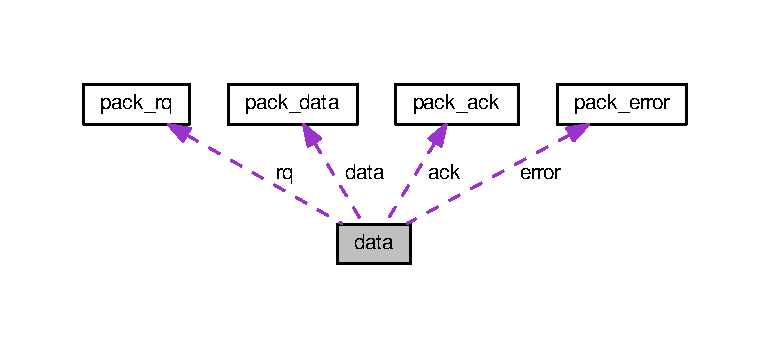
\includegraphics[width=350pt]{uniondata__coll__graph}
\end{center}
\end{figure}
\subsection*{Public Attributes}
\begin{DoxyCompactItemize}
\item 
struct \hyperlink{structpack__rq}{pack\+\_\+rq} {\bfseries rq}\hypertarget{uniondata_acf4172048a0f6d3c7259374b38040c62}{}\label{uniondata_acf4172048a0f6d3c7259374b38040c62}

\item 
struct \hyperlink{structpack__data}{pack\+\_\+data} {\bfseries data}\hypertarget{uniondata_a729b3758577c1e6f2b5ce2325a4dc49b}{}\label{uniondata_a729b3758577c1e6f2b5ce2325a4dc49b}

\item 
struct \hyperlink{structpack__ack}{pack\+\_\+ack} {\bfseries ack}\hypertarget{uniondata_a0b33fddc0ac4377dc9d7f21987686417}{}\label{uniondata_a0b33fddc0ac4377dc9d7f21987686417}

\item 
struct \hyperlink{structpack__error}{pack\+\_\+error} {\bfseries error}\hypertarget{uniondata_a633fcc64b90ce21b13b425987a6e78b8}{}\label{uniondata_a633fcc64b90ce21b13b425987a6e78b8}

\end{DoxyCompactItemize}


The documentation for this union was generated from the following file\+:\begin{DoxyCompactItemize}
\item 
src/lib/\hyperlink{tftp_8h}{tftp.\+h}\end{DoxyCompactItemize}

\hypertarget{structpack__ack}{}\section{pack\+\_\+ack Struct Reference}
\label{structpack__ack}\index{pack\+\_\+ack@{pack\+\_\+ack}}
\subsection*{Public Attributes}
\begin{DoxyCompactItemize}
\item 
uint16\+\_\+t {\bfseries block}\hypertarget{structpack__ack_afa1589b04941d35081b8c4577103a23c}{}\label{structpack__ack_afa1589b04941d35081b8c4577103a23c}

\end{DoxyCompactItemize}


The documentation for this struct was generated from the following file\+:\begin{DoxyCompactItemize}
\item 
src/lib/\hyperlink{tftp_8h}{tftp.\+h}\end{DoxyCompactItemize}

\hypertarget{structpack__data}{}\section{pack\+\_\+data Struct Reference}
\label{structpack__data}\index{pack\+\_\+data@{pack\+\_\+data}}
\subsection*{Public Attributes}
\begin{DoxyCompactItemize}
\item 
uint16\+\_\+t {\bfseries block}\hypertarget{structpack__data_a068c6d09f17d908c17125d340ce6d395}{}\label{structpack__data_a068c6d09f17d908c17125d340ce6d395}

\item 
char {\bfseries data} \mbox{[}512\mbox{]}\hypertarget{structpack__data_a8544d11ed274e1889f67d2451fe6906d}{}\label{structpack__data_a8544d11ed274e1889f67d2451fe6906d}

\end{DoxyCompactItemize}


The documentation for this struct was generated from the following file\+:\begin{DoxyCompactItemize}
\item 
src/lib/\hyperlink{tftp_8h}{tftp.\+h}\end{DoxyCompactItemize}

\hypertarget{structpack__error}{}\section{pack\+\_\+error Struct Reference}
\label{structpack__error}\index{pack\+\_\+error@{pack\+\_\+error}}
\subsection*{Public Attributes}
\begin{DoxyCompactItemize}
\item 
uint16\+\_\+t {\bfseries ercode}\hypertarget{structpack__error_a2277d88f47761ca35420f75ec268414e}{}\label{structpack__error_a2277d88f47761ca35420f75ec268414e}

\item 
char $\ast$ {\bfseries msg}\hypertarget{structpack__error_a9922c5ce6ba29d4df94bab403e8b226b}{}\label{structpack__error_a9922c5ce6ba29d4df94bab403e8b226b}

\end{DoxyCompactItemize}


The documentation for this struct was generated from the following file\+:\begin{DoxyCompactItemize}
\item 
src/lib/\hyperlink{tftp_8h}{tftp.\+h}\end{DoxyCompactItemize}

\hypertarget{structpack__rq}{}\section{pack\+\_\+rq Struct Reference}
\label{structpack__rq}\index{pack\+\_\+rq@{pack\+\_\+rq}}
\subsection*{Public Attributes}
\begin{DoxyCompactItemize}
\item 
char $\ast$ {\bfseries filename}\hypertarget{structpack__rq_a622b8df02698132010c1be70b3c4800c}{}\label{structpack__rq_a622b8df02698132010c1be70b3c4800c}

\item 
char $\ast$ {\bfseries mode}\hypertarget{structpack__rq_a9db298cebff7089a3a4d51957d4e09ac}{}\label{structpack__rq_a9db298cebff7089a3a4d51957d4e09ac}

\end{DoxyCompactItemize}


The documentation for this struct was generated from the following file\+:\begin{DoxyCompactItemize}
\item 
src/lib/\hyperlink{tftp_8h}{tftp.\+h}\end{DoxyCompactItemize}

\hypertarget{structtftp__pack__s}{}\section{tftp\+\_\+pack\+\_\+s Struct Reference}
\label{structtftp__pack__s}\index{tftp\+\_\+pack\+\_\+s@{tftp\+\_\+pack\+\_\+s}}


{\ttfamily \#include $<$tftp.\+h$>$}



Collaboration diagram for tftp\+\_\+pack\+\_\+s\+:\nopagebreak
\begin{figure}[H]
\begin{center}
\leavevmode
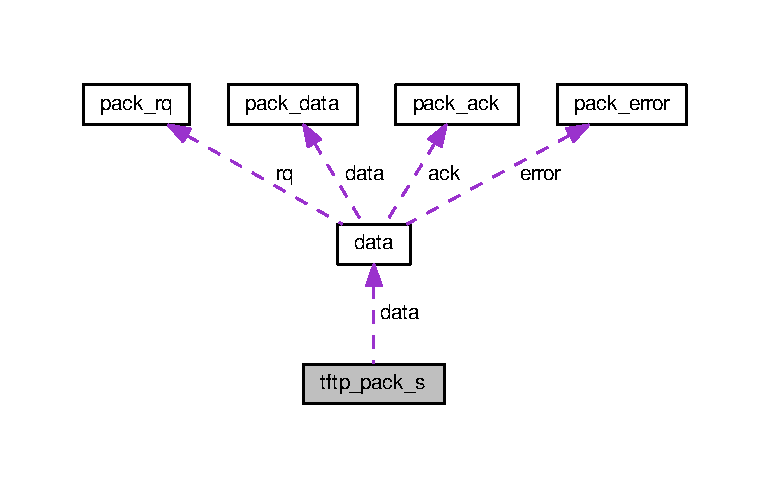
\includegraphics[width=350pt]{structtftp__pack__s__coll__graph}
\end{center}
\end{figure}
\subsection*{Public Attributes}
\begin{DoxyCompactItemize}
\item 
uint16\+\_\+t {\bfseries opcode}\hypertarget{structtftp__pack__s_a20c790cca5e1780bd0b37076f5be37ce}{}\label{structtftp__pack__s_a20c790cca5e1780bd0b37076f5be37ce}

\item 
union \hyperlink{uniondata}{data} $\ast$ {\bfseries data}\hypertarget{structtftp__pack__s_a4c5e82ec1216b1b1c258fd34688f66ae}{}\label{structtftp__pack__s_a4c5e82ec1216b1b1c258fd34688f66ae}

\end{DoxyCompactItemize}


\subsection{Detailed Description}
T\+F\+TP packet structure. 

The documentation for this struct was generated from the following file\+:\begin{DoxyCompactItemize}
\item 
src/lib/\hyperlink{tftp_8h}{tftp.\+h}\end{DoxyCompactItemize}

\chapter{File Documentation}
\hypertarget{tftp_8c}{}\section{src/lib/tftp.c File Reference}
\label{tftp_8c}\index{src/lib/tftp.\+c@{src/lib/tftp.\+c}}


T\+F\+TP protocol library.  


{\ttfamily \#include \char`\"{}tftp.\+h\char`\"{}}\\*
{\ttfamily \#include $<$apr\+\_\+strings.\+h$>$}\\*
{\ttfamily \#include $<$stdio.\+h$>$}\\*
Include dependency graph for tftp.\+c\+:\nopagebreak
\begin{figure}[H]
\begin{center}
\leavevmode
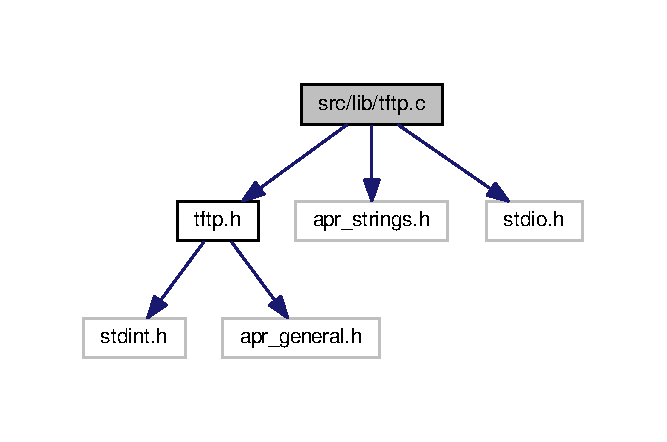
\includegraphics[width=320pt]{tftp_8c__incl}
\end{center}
\end{figure}
\subsection*{Functions}
\begin{DoxyCompactItemize}
\item 
\hyperlink{structtftp__pack__s}{tftp\+\_\+pack} $\ast$ \hyperlink{tftp_8c_af6ff5c665916da8a6f7b1d844f91bab9}{tftp\+\_\+packet\+\_\+read} (char $\ast$packet, apr\+\_\+size\+\_\+t len, apr\+\_\+pool\+\_\+t $\ast$mp)
\end{DoxyCompactItemize}


\subsection{Detailed Description}
T\+F\+TP protocol library. 

tftpclient -- T\+F\+TP client application. Copyright (C) 2016, Stas Kobzar \href{mailto:staskobzar@modulis.ca}{\tt staskobzar@modulis.\+ca}

This file is part of tftpclient.

tftpclient is free software\+: you can redistribute it and/or modify it under the terms of the G\+NU General Public License as published by the Free Software Foundation, either version 3 of the License, or (at your option) any later version.

tftpclient is distributed in the hope that it will be useful, but W\+I\+T\+H\+O\+UT A\+NY W\+A\+R\+R\+A\+N\+TY; without even the implied warranty of M\+E\+R\+C\+H\+A\+N\+T\+A\+B\+I\+L\+I\+TY or F\+I\+T\+N\+E\+SS F\+OR A P\+A\+R\+T\+I\+C\+U\+L\+AR P\+U\+R\+P\+O\+SE. See the G\+NU General Public License for more details.

You should have received a copy of the G\+NU General Public License along with tftpclient. If not, see \href{http://www.gnu.org/licenses/}{\tt http\+://www.\+gnu.\+org/licenses/}.

\begin{DoxyAuthor}{Author}
Stas Kobzar \href{mailto:staskobzar@gmail.com}{\tt staskobzar@gmail.\+com} 
\end{DoxyAuthor}


\subsection{Function Documentation}
\index{tftp.\+c@{tftp.\+c}!tftp\+\_\+packet\+\_\+read@{tftp\+\_\+packet\+\_\+read}}
\index{tftp\+\_\+packet\+\_\+read@{tftp\+\_\+packet\+\_\+read}!tftp.\+c@{tftp.\+c}}
\subsubsection[{\texorpdfstring{tftp\+\_\+packet\+\_\+read(char $\ast$packet, apr\+\_\+size\+\_\+t len, apr\+\_\+pool\+\_\+t $\ast$mp)}{tftp_packet_read(char *packet, apr_size_t len, apr_pool_t *mp)}}]{\setlength{\rightskip}{0pt plus 5cm}{\bf tftp\+\_\+pack}$\ast$ tftp\+\_\+packet\+\_\+read (
\begin{DoxyParamCaption}
\item[{char $\ast$}]{packet, }
\item[{apr\+\_\+size\+\_\+t}]{len, }
\item[{apr\+\_\+pool\+\_\+t $\ast$}]{mp}
\end{DoxyParamCaption}
)}\hypertarget{tftp_8c_af6ff5c665916da8a6f7b1d844f91bab9}{}\label{tftp_8c_af6ff5c665916da8a6f7b1d844f91bab9}
Read tftp packet received from socket. 
\begin{DoxyParams}{Parameters}
{\em packet} & T\+F\+TP packet \\
\hline
{\em len} & Packet length \\
\hline
{\em mp} & A\+PR memory pool \\
\hline
\end{DoxyParams}
\begin{DoxyReturn}{Returns}
tftp\+\_\+pack struct 
\end{DoxyReturn}

\hypertarget{tftp_8h}{}\section{src/lib/tftp.h File Reference}
\label{tftp_8h}\index{src/lib/tftp.\+h@{src/lib/tftp.\+h}}


T\+F\+TP protocol library.  


{\ttfamily \#include $<$stdint.\+h$>$}\\*
{\ttfamily \#include $<$apr\+\_\+general.\+h$>$}\\*
Include dependency graph for tftp.\+h\+:\nopagebreak
\begin{figure}[H]
\begin{center}
\leavevmode
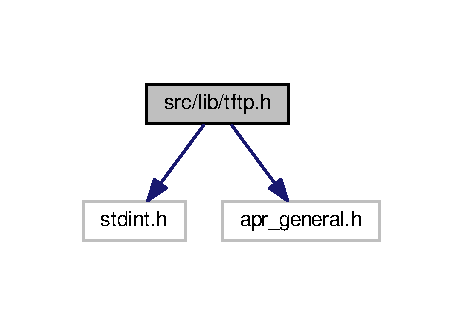
\includegraphics[width=222pt]{tftp_8h__incl}
\end{center}
\end{figure}
This graph shows which files directly or indirectly include this file\+:\nopagebreak
\begin{figure}[H]
\begin{center}
\leavevmode
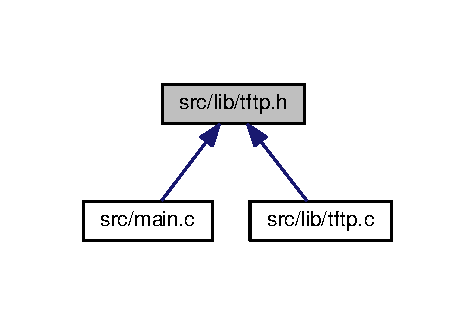
\includegraphics[width=228pt]{tftp_8h__dep__incl}
\end{center}
\end{figure}
\subsection*{Classes}
\begin{DoxyCompactItemize}
\item 
struct \hyperlink{structpack__rq}{pack\+\_\+rq}
\item 
struct \hyperlink{structpack__data}{pack\+\_\+data}
\item 
struct \hyperlink{structpack__ack}{pack\+\_\+ack}
\item 
struct \hyperlink{structpack__error}{pack\+\_\+error}
\item 
union \hyperlink{uniondata}{data}
\item 
struct \hyperlink{structtftp__pack__s}{tftp\+\_\+pack\+\_\+s}
\end{DoxyCompactItemize}
\subsection*{Macros}
\begin{DoxyCompactItemize}
\item 
\#define {\bfseries M\+O\+D\+E\+\_\+\+O\+C\+T\+ET}~\char`\"{}octet\char`\"{}\hypertarget{tftp_8h_a1c7eacf19a40f0a1dec5768b3713fd39}{}\label{tftp_8h_a1c7eacf19a40f0a1dec5768b3713fd39}

\item 
\#define {\bfseries M\+O\+D\+E\+\_\+\+A\+S\+C\+II}~\char`\"{}netascii\char`\"{}\hypertarget{tftp_8h_af3daaf7e450c6eefe8e2d8c24b797661}{}\label{tftp_8h_af3daaf7e450c6eefe8e2d8c24b797661}

\item 
\#define {\bfseries M\+O\+D\+E\+\_\+\+M\+A\+IL}~\char`\"{}mail\char`\"{}\hypertarget{tftp_8h_a235fc109418aaef8b068f77314e3b598}{}\label{tftp_8h_a235fc109418aaef8b068f77314e3b598}

\end{DoxyCompactItemize}
\subsection*{Typedefs}
\begin{DoxyCompactItemize}
\item 
typedef struct \hyperlink{structtftp__pack__s}{tftp\+\_\+pack\+\_\+s} {\bfseries tftp\+\_\+pack}\hypertarget{tftp_8h_a6706b3408d5dd262fde30dc6b1bc1700}{}\label{tftp_8h_a6706b3408d5dd262fde30dc6b1bc1700}

\end{DoxyCompactItemize}
\subsection*{Enumerations}
\begin{DoxyCompactItemize}
\item 
enum {\bfseries opcodes} \{ \\*
{\bfseries E\+\_\+\+R\+RQ} = 0x01, 
{\bfseries E\+\_\+\+W\+RQ} = 0x02, 
{\bfseries E\+\_\+\+D\+A\+TA} = 0x03, 
{\bfseries E\+\_\+\+A\+CK} = 0x04, 
\\*
{\bfseries E\+\_\+\+E\+R\+R\+OR} = 0x05
 \}\hypertarget{tftp_8h_a44c68a04cafe3d38456832196c7bf22a}{}\label{tftp_8h_a44c68a04cafe3d38456832196c7bf22a}

\end{DoxyCompactItemize}
\subsection*{Functions}
\begin{DoxyCompactItemize}
\item 
\hyperlink{structtftp__pack__s}{tftp\+\_\+pack} $\ast$ \hyperlink{tftp_8h_af6ff5c665916da8a6f7b1d844f91bab9}{tftp\+\_\+packet\+\_\+read} (char $\ast$packet, apr\+\_\+size\+\_\+t len, apr\+\_\+pool\+\_\+t $\ast$mp)
\end{DoxyCompactItemize}


\subsection{Detailed Description}
T\+F\+TP protocol library. 

tftpclient -- T\+F\+TP client application. Copyright (C) 2016, Stas Kobzar \href{mailto:staskobzar@modulis.ca}{\tt staskobzar@modulis.\+ca}

This file is part of tftpclient.

tftpclient is free software\+: you can redistribute it and/or modify it under the terms of the G\+NU General Public License as published by the Free Software Foundation, either version 3 of the License, or (at your option) any later version.

tftpclient is distributed in the hope that it will be useful, but W\+I\+T\+H\+O\+UT A\+NY W\+A\+R\+R\+A\+N\+TY; without even the implied warranty of M\+E\+R\+C\+H\+A\+N\+T\+A\+B\+I\+L\+I\+TY or F\+I\+T\+N\+E\+SS F\+OR A P\+A\+R\+T\+I\+C\+U\+L\+AR P\+U\+R\+P\+O\+SE. See the G\+NU General Public License for more details.

You should have received a copy of the G\+NU General Public License along with tftpclient. If not, see \href{http://www.gnu.org/licenses/}{\tt http\+://www.\+gnu.\+org/licenses/}.

\begin{DoxyAuthor}{Author}
Stas Kobzar \href{mailto:staskobzar@gmail.com}{\tt staskobzar@gmail.\+com} 
\end{DoxyAuthor}


\subsection{Function Documentation}
\index{tftp.\+h@{tftp.\+h}!tftp\+\_\+packet\+\_\+read@{tftp\+\_\+packet\+\_\+read}}
\index{tftp\+\_\+packet\+\_\+read@{tftp\+\_\+packet\+\_\+read}!tftp.\+h@{tftp.\+h}}
\subsubsection[{\texorpdfstring{tftp\+\_\+packet\+\_\+read(char $\ast$packet, apr\+\_\+size\+\_\+t len, apr\+\_\+pool\+\_\+t $\ast$mp)}{tftp_packet_read(char *packet, apr_size_t len, apr_pool_t *mp)}}]{\setlength{\rightskip}{0pt plus 5cm}{\bf tftp\+\_\+pack}$\ast$ tftp\+\_\+packet\+\_\+read (
\begin{DoxyParamCaption}
\item[{char $\ast$}]{packet, }
\item[{apr\+\_\+size\+\_\+t}]{len, }
\item[{apr\+\_\+pool\+\_\+t $\ast$}]{mp}
\end{DoxyParamCaption}
)}\hypertarget{tftp_8h_af6ff5c665916da8a6f7b1d844f91bab9}{}\label{tftp_8h_af6ff5c665916da8a6f7b1d844f91bab9}
Read tftp packet received from socket. 
\begin{DoxyParams}{Parameters}
{\em packet} & T\+F\+TP packet \\
\hline
{\em len} & Packet length \\
\hline
{\em mp} & A\+PR memory pool \\
\hline
\end{DoxyParams}
\begin{DoxyReturn}{Returns}
tftp\+\_\+pack struct 
\end{DoxyReturn}

\hypertarget{main_8c}{}\section{src/main.c File Reference}
\label{main_8c}\index{src/main.\+c@{src/main.\+c}}


tftpclient main proc  


{\ttfamily \#include \char`\"{}tftp.\+h\char`\"{}}\\*
{\ttfamily \#include \char`\"{}util.\+h\char`\"{}}\\*
{\ttfamily \#include $<$stdio.\+h$>$}\\*
Include dependency graph for main.\+c\+:\nopagebreak
\begin{figure}[H]
\begin{center}
\leavevmode
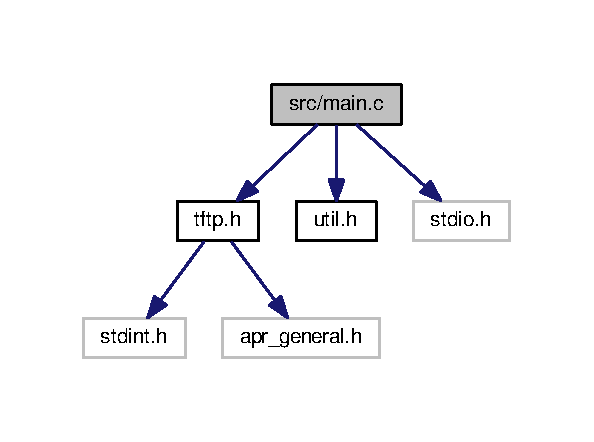
\includegraphics[width=285pt]{main_8c__incl}
\end{center}
\end{figure}
\subsection*{Functions}
\begin{DoxyCompactItemize}
\item 
int {\bfseries main} (int argc, const char $\ast$argv\mbox{[}$\,$\mbox{]})\hypertarget{main_8c_ac0f2228420376f4db7e1274f2b41667c}{}\label{main_8c_ac0f2228420376f4db7e1274f2b41667c}

\end{DoxyCompactItemize}


\subsection{Detailed Description}
tftpclient main proc 

tftpclient -- T\+F\+TP client application. Copyright (C) 2016, Stas Kobzar \href{mailto:staskobzar@modulis.ca}{\tt staskobzar@modulis.\+ca}

This file is part of tftpclient.

tftpclient is free software\+: you can redistribute it and/or modify it under the terms of the G\+NU General Public License as published by the Free Software Foundation, either version 3 of the License, or (at your option) any later version.

tftpclient is distributed in the hope that it will be useful, but W\+I\+T\+H\+O\+UT A\+NY W\+A\+R\+R\+A\+N\+TY; without even the implied warranty of M\+E\+R\+C\+H\+A\+N\+T\+A\+B\+I\+L\+I\+TY or F\+I\+T\+N\+E\+SS F\+OR A P\+A\+R\+T\+I\+C\+U\+L\+AR P\+U\+R\+P\+O\+SE. See the G\+NU General Public License for more details.

You should have received a copy of the G\+NU General Public License along with tftpclient. If not, see \href{http://www.gnu.org/licenses/}{\tt http\+://www.\+gnu.\+org/licenses/}.

\begin{DoxyAuthor}{Author}
Stas Kobzar \href{mailto:staskobzar@gmail.com}{\tt staskobzar@gmail.\+com} 
\end{DoxyAuthor}

\hypertarget{util_8c}{}\section{src/util.c File Reference}
\label{util_8c}\index{src/util.\+c@{src/util.\+c}}


tftpclient utilities functions  




\subsection{Detailed Description}
tftpclient utilities functions 

tftpclient -- T\+F\+TP client application. Copyright (C) 2016, Stas Kobzar \href{mailto:staskobzar@modulis.ca}{\tt staskobzar@modulis.\+ca}

This file is part of tftpclient.

tftpclient is free software\+: you can redistribute it and/or modify it under the terms of the G\+NU General Public License as published by the Free Software Foundation, either version 3 of the License, or (at your option) any later version.

tftpclient is distributed in the hope that it will be useful, but W\+I\+T\+H\+O\+UT A\+NY W\+A\+R\+R\+A\+N\+TY; without even the implied warranty of M\+E\+R\+C\+H\+A\+N\+T\+A\+B\+I\+L\+I\+TY or F\+I\+T\+N\+E\+SS F\+OR A P\+A\+R\+T\+I\+C\+U\+L\+AR P\+U\+R\+P\+O\+SE. See the G\+NU General Public License for more details.

You should have received a copy of the G\+NU General Public License along with tftpclient. If not, see \href{http://www.gnu.org/licenses/}{\tt http\+://www.\+gnu.\+org/licenses/}.

\begin{DoxyAuthor}{Author}
Stas Kobzar \href{mailto:staskobzar@gmail.com}{\tt staskobzar@gmail.\+com} 
\end{DoxyAuthor}

\hypertarget{util_8h}{}\section{src/util.h File Reference}
\label{util_8h}\index{src/util.\+h@{src/util.\+h}}


tftpclient utilities function  


This graph shows which files directly or indirectly include this file\+:\nopagebreak
\begin{figure}[H]
\begin{center}
\leavevmode
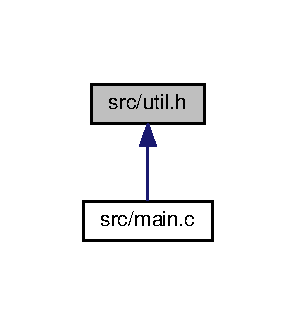
\includegraphics[width=142pt]{util_8h__dep__incl}
\end{center}
\end{figure}


\subsection{Detailed Description}
tftpclient utilities function 

tftpclient -- T\+F\+TP client application. Copyright (C) 2016, Stas Kobzar \href{mailto:staskobzar@modulis.ca}{\tt staskobzar@modulis.\+ca}

This file is part of tftpclient.

tftpclient is free software\+: you can redistribute it and/or modify it under the terms of the G\+NU General Public License as published by the Free Software Foundation, either version 3 of the License, or (at your option) any later version.

tftpclient is distributed in the hope that it will be useful, but W\+I\+T\+H\+O\+UT A\+NY W\+A\+R\+R\+A\+N\+TY; without even the implied warranty of M\+E\+R\+C\+H\+A\+N\+T\+A\+B\+I\+L\+I\+TY or F\+I\+T\+N\+E\+SS F\+OR A P\+A\+R\+T\+I\+C\+U\+L\+AR P\+U\+R\+P\+O\+SE. See the G\+NU General Public License for more details.

You should have received a copy of the G\+NU General Public License along with tftpclient. If not, see \href{http://www.gnu.org/licenses/}{\tt http\+://www.\+gnu.\+org/licenses/}.

\begin{DoxyAuthor}{Author}
Stas Kobzar \href{mailto:staskobzar@gmail.com}{\tt staskobzar@gmail.\+com} 
\end{DoxyAuthor}

%--- End generated contents ---

% Index
\backmatter
\newpage
\phantomsection
\clearemptydoublepage
\addcontentsline{toc}{chapter}{Index}
\printindex

\end{document}
